	
\documentclass[review]{elsarticle}
\usepackage{hyperref,lineno}
\usepackage{xcolor}
\modulolinenumbers[5]

\newcommand{\memo}[2]{\textcolor{#1}{#2}}
\newcommand{\xavi}[1]{\memo{orange}{xavi: #1\\}}
\newcommand{\maria}[1]{\memo{blue}{maria: #1\\}}
\journal{Journal of \LaTeX\ Templates}

%%%%%%%%%%%%%%%%%%%%%%%
%% Elsevier bibliography styles
%%%%%%%%%%%%%%%%%%%%%%%
%% To change the style, put a % in front of the second line of the current style and
%% remove the % from the second line of the style you would like to use.
%%%%%%%%%%%%%%%%%%%%%%%

%% Numbered
%\bibliographystyle{model1-num-names}

%% Numbered without titles
%\bibliographystyle{model1a-num-names}

%% Harvard
\bibliographystyle{model2-names.bst}\biboptions{authoryear}

%% Vancouver numbered
%\usepackage{numcompress}\bibliographystyle{model3-num-names}

%% Vancouver name/year
%\usepackage{numcompress}\bibliographystyle{model4-names}\biboptions{authoryear}

%% APA style
%\bibliographystyle{model5-names}\biboptions{authoryear}

%% AMA style
%\usepackage{numcompress}\bibliographystyle{model6-num-names}

%% `Elsevier LaTeX' style
%\bibliographystyle{elsarticle-num}
%%%%%%%%%%%%%%%%%%%%%%%

\begin{document}

\begin{frontmatter}

\title{Identifying social learning between Roman amphorae workshops through morphometric similarity}

%% Group authors per affiliation:
%\author{Mar\'ia Coto-Sarmiento\fnref{myfootnot}}
\author[bscadress]{Maria Coto-Sarmiento\corref{mycorrespondingauthor}}
\cortext[mycorrespondingauthor]{Corresponding author}
\ead{maria.coto@bsc.es}


\author[edadress]{Xavier Rubio-Campillo}
\author[ceipacadress]{Jos\'e Remesal}

%\address{Radarweg 29, Amsterdam}
%\fntext[myfootnote]{Since 1880.}

%% or include affiliations in footnotes:
%\author[mymainaddress,mysecondaryaddress]{Elsevier Inc}
%\ead[url]{www.elsevier.com}

%\author[mysecondaryaddress]{Maria Coto-Sarmiento\corref{mycorrespondingauthor}}

\address[bscadress]{Barcelona Supercomputing Center (BSC), Jordi Girona 29, Office 3A, Nexus II Building, 08034, Barcelona, Spain}
\address[edadress]{School of History, Classic \& Archaeology, Room OOM.22, William Robertson Wing, Old Medical School, Teviot Place, University of Edinburgh, UK}
\address[ceipacadress]{CEIPAC, Department of Prehistory and Archaeology, Montalegre, 6-8, 08001, University of Barcelona, Barcelona, Spain}

\begin{abstract}

The aim of this study is to identify interactive dynamics within amphorae workshops in the Roman Empire. The \textit{Baetica} province (currently Andalusia, southern Spain) hosted for almost 300 years a massive infrastructure that supplied olive oil to the Western provinces of Rome. A large number of workshops produced the same type of amphora to ship the product through maritime and riverine transport networks. Despite the amount of evidence it is difficult to find an archaeological proxy able to tell us how were these workshops organised.

We apply here an evolutionary framework to understand potential links between workshops through morphometric similarities in the amphorae they produced. By exploring small yet statistical significant differences in the amphorae made in 5 different workshops the approach is able to identify how individual potters acquired and transmitted technical skills.  Our approach applies multivariate statistical methods to cluster a variety of amphorae based on morphometric measurements. Other studies have developed similar approach to analyse handmade pottery but we show here that the method can be also applied to large-scale production of a standardized amphora type (i.e. Dressel 20).

Results suggest that morphometric similarity is inversely correlated with spatial distance between workshops. This outcome suggests that pottery-making techniques were transmited through vertical transmission with little or no movement of potters between distant workshops. The work also highlights that morphometric similarity may be an effective proxy to identify social learning dynamics even amongst workshops producing exactly the same amphoric type. 

\end{abstract}

\begin{keyword}
Roman Empire, amphorae, Dressel 20, social learning, cultural evolution
\end{keyword}

\end{frontmatter}

\linenumbers

%\section{The Elsevier article class}

%\paragraph{Installation} If the document class \emph{elsarticle} is not available on your computer, you can download and install the system package \emph{texlive-publishers} (Linux) or the \LaTeX\ package \emph{elsarticle} using the package manager of your \TeX\ installation, which is typically \TeX\ Live or Mik\TeX.

%\paragraph{Usage} Once the package is properly installed, you can use the document class \emph{elsarticle} to create a manuscript. Please make sure that your manuscript follows the guidelines in the Guide for Authors of the relevant journal. It is not necessary to typeset your manuscript in exactly the same way as an article, unless you are submitting to a camera-ready copy (CRC) journal.

%\paragraph{Functionality} The Elsevier article class is based on the standard article class and supports almost all of the functionality of that class. In addition, it features commands and options to format the
%\begin{itemize}
%\item document style
%\item baselineskip
%\item front matter
%\item keywords and MSC codes
%\item theorems, definitions and proofs
%\item lables of enumerations
%\item citation style and labeling.
%\end{itemize}

%\section{Front matter}
%The author names and affiliations could be formatted in two ways:
%\begin{enumerate}[(1)]
%\item Group the authors per affiliation.
%\item Use footnotes to indicate the affiliations.
%\end{enumerate}
%See the front matter of this document for examples. You are recommended to conform your choice to the journal you are submitting to.


\section{Introduction}

The archaeological record can help us identify the mechanisms by which humans learn from each other~\citep{richerson2005not,schillinger_copying_2016}. Cultural transmission dynamics can be identified by analysing archaeological proxies able to capture the distinct variability generated by different social learning mechanisms~\citep{shennan_ceramic_2001,eerkens_jelmer_cultural_2005}. This approach has been succesfully applied to the material culture generated by small-scale societies but it has been seldom explored in the case of large-scale production~\citep{shennan_isolation-by-distance_2015,neff1992ceramics}.

This paper explores the social dynamics of specialized production in the Roman Empire. Wwe focus here on analysing large-scale production of a single amphoric type (Dressel 20) in a specific area. An evolutionary framework has been used to identify social learning dynamics between pottery-makers \citep{mesoudi_cultural_2015, shennan_evolution_2008}. Following a large number of authors \citep{cavalli-sforza_cultural_1981, hosfield_modes_2009}, pottery production can be learned on different modes of cultural transmission depending on the level of production in the communities. Vertical transmission is a mode of transmission when the teaching of the production is done from master to disciple while in horizontal transmission individuals teach pottery techniques to other individuals within the same level and those workers spread the knowledge to their community \citep{epstein_craft_1998}.

Artefact variation should also be affected by geographical distance \citep{bjorklund_effect_2010,shennan_isolation-by-distance_2015, van_strien_isolation-by-distance_2015}. If vertical transmission is predominant then culture should be similar in nearby groups with high degrees of interaction \citep{hart_effects_2012}. The underlying consequence is that it should be possible to identify interaction between workshops by quantifying similarity amongst the amphorae they produced; if apprentices moved between distant workshops then no differences would be found on this proxy while a more strict vertical transmission would be revealed by distant workshops exhibiting less similarity.


%Specifically, the aim of this study is understanding if pottery-making techniques were transmitted through vertical or horizontal social learning. Our main hypothesis concerns the transmission of the techniques by vertical transmission and how vertical transmission is spreading in time and space. These technological knowledges could have been transmitted from master to disciple and thus continuously. If vertical transmission predominates in this process over horizontal transmission then amphorae made in nearby workshops might share more similar traits than amphorae made from farthest workshop. Otherwise whether horizontal transmission is the main transmission in this process the social learning would be transmitted by workers. Then there would not be differences among workshops on the production. The artefact variation can be related to the geographical distance \citep{bjorklund_effect_2010,shennan_isolation-by-distance_2015, van_strien_isolation-by-distance_2015}. In material culture, artefact variation might be affected by geographical distance where material culture is more similar in close population who interacted each other. In other case, the correlation between both seems not visible due to different factors \citep{hart_effects_2012}. In our case, we can detect measurable differences among this type of amphorae correlated with the geographical distance.

The debate on social learning processes is hindered by the challenge of detecting the different modes of transmission in the archaeological record \citep{roux_standardization_2015}. In the case of archaeology, several studies have analysed this process focused on the production of handmade pottery \citep{steele_james_ceramic_2010} or with stylistic variations \citep{neiman_stylistic_1995, shennan_ceramic_2001}. Our work aims at identifying learning processes even in the case of the standardized massive olive oil production common during the Roman Empire \citep{gandon_copying_2014,bevan_mediterranean_2014}. 

Olive oil was one of the most important products of the Classical Mediterranean world as it was used in almost all aspects of daily life including cooking, lightning and hygiene \citep{mattingly_d.j._oil_1988}. The \emph{Baetica} province (currently Andalusia, southern Spain) developed a massive infrastructure of olive oil production to face the demands of the Roman Empire. The product was shipped in large amounts of amphorae to distant provinces all along the Western provinces. One of its most important clients was the Roman army as olive oil was supplied to tens of thousands of legionaries in places such as Britania \citep{funari_economic_2005, monfort_britannia_1998} and Germania \citep{remesal_annona_1986}. 

For this reason, this ancient province became an important support for the production and distribution of olive oil to the rest of the Empire during three centuries \citep{chic2005comercio, millet_anforas_1998, rodriguez_baetican_1998}. \emph{Baetica} provided a strong connectivity through riverine transport that allowed inland producers to use an important trade network through the Mediterranean and Atlantic \citep{garcia_vargas_enrique_formal_2010}. The exponential production growth required the creation of over a hundred amphora workshops supporting olive oil shipment. These workshops were located along the Guadalquivir river and its tributaries. The majority of amphorae produced in this area are classified as \emph{Dressel 20} type divided into a variety of subclasses \citep{berni_millet_epigrafianforica_2008, martin-kilcher_romischen_1994}. Dressel 20 were used mostly to transport olive oil for around 300 years in order to satisfy the demand within Roman Empire \citep{rodriguez_economioleicola_1977}. 

% For example, Dressel 20 amphora often displayed a stamp identifying an economic actor involved in the production \citep{coto-sarmiento_maria_bayesian_????}.
This specialized production was highly standardized both in terms of products and processes and did not vary much. The same type of amphora was produced over 300 years with small differences while similar stamps and information was recorded on them \cite{coto-sarmiento_maria_bayesian_????}. Despite our knowledge of the process little is known on how learning was organised in these workshops. Did they have different traditions and apprentices worked in the place where they were trained? Did potters work in more than one workshop? Were changes in production decided by workshops or by external actors? All these questions are linked to the social learning processes that took place in the workshops. If the system was organised based on vertical transmission mechanisms with no potters moving to distant workshops then amphorae produced in nearby workshops might share more similar traits than with the rest of the production. On the other hand, if horizontal dynamics were common then this correlation with spatial coordinates should not be present as workers would share their methods \citep{hosfield_modes_2009}. 

The paper can be summarized as follows. The next section introduces the dataset and the methods used to analyse it. Section three presents the results while the last part discusses the outcomes and highlights the main conclusions of the work. 

\section{Material and methods}

Our sample consisted of 413 Dressel 20 amphorae collected from the 5 Dressel 20 workshops that have been more intensively excavated in the last 4 decades. The workshops were located at Malpica, Cerro del Bel\'en (hereafter, Bel\'en) \citep{diaz_trujillo_excavacion_1992}, Parlamento \citep{garcia_vargas_anforas_2000}, Villaseca\citep{garcia_vargas_enrique_excavacion_????} and Las Delicias \citep{fernandez_excavacion_2001,_atelier_2014} (see Figure \ref{romanworkshop}).

\begin{figure}[htp]
	\centering
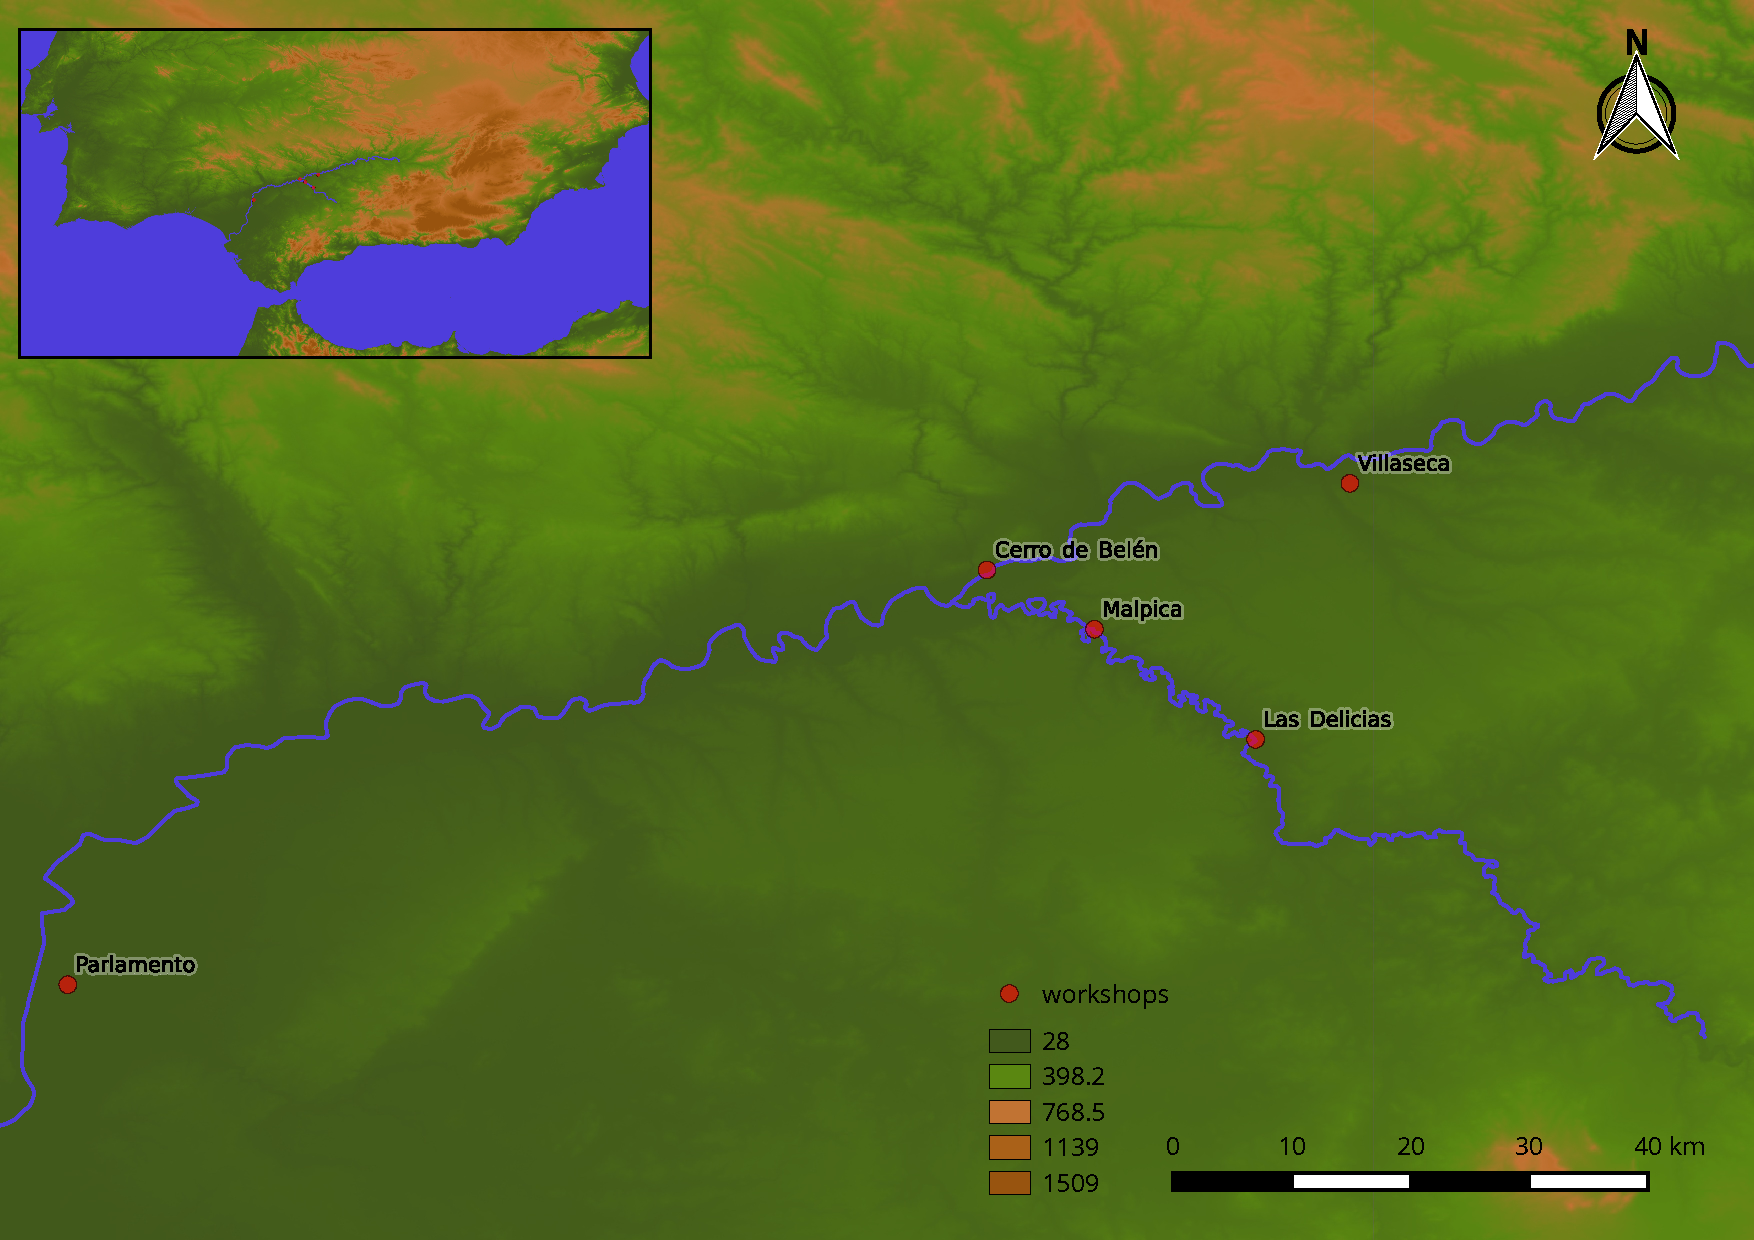
\includegraphics[width=\linewidth]{figs/romanworkshop}
\caption{Map from \textit{Baetica} province during the Roman Empire depicting the location of the 5 analyzed workshops. Dressel 20 workshops were mostly distributed along the rivers Gualdalquivir and Genil.}
\label{romanworkshop}
\end{figure} 

The sample was roughly uniformly distributed amongst the 5 workshops (80-100 samples for each of them). These workshops were located a diversity of locations so spatial dynamics could be potentially identified. All of them had overlapping long chronologies so differences in amphorae could not be inherently explained by temporal variation. This trait is reinforced by the fact that the Dressel 20 type did not show any remarkable change in shape for almost three centuries \citep{berni_dressel_2016}. We analyzed Dressel 20 of the three most abundant variants spanning three centuries (Dressel C, Dressel D, Dressel E) \citep{berni_millet_epigrafianforica_2008,martin-kilcher_romischen_1994}. All the variants were found in the 5 workshops so no intrinsic bias was generated by them. 

Eight different measurements were taken from each amphora. The metrics were focused on the rim sherds as this section presents the best preservation for most archaeological contexts and they present good indicators of variation \citep{berni_millet_epigrafianforica_2008}. Other interesting proxiies such as handles and bases were found in lesser quantities and for this reason they would be less useful for quantitative approaches due to low sample size. The measurements can be seen in Figureg~\ref{mesures}; they were divided into exterior diameter, inside diameter, rim height, rim width, shape width, rim inside height, rim width 2 and protruding rim.

\begin{figure}[htp]
	\centering
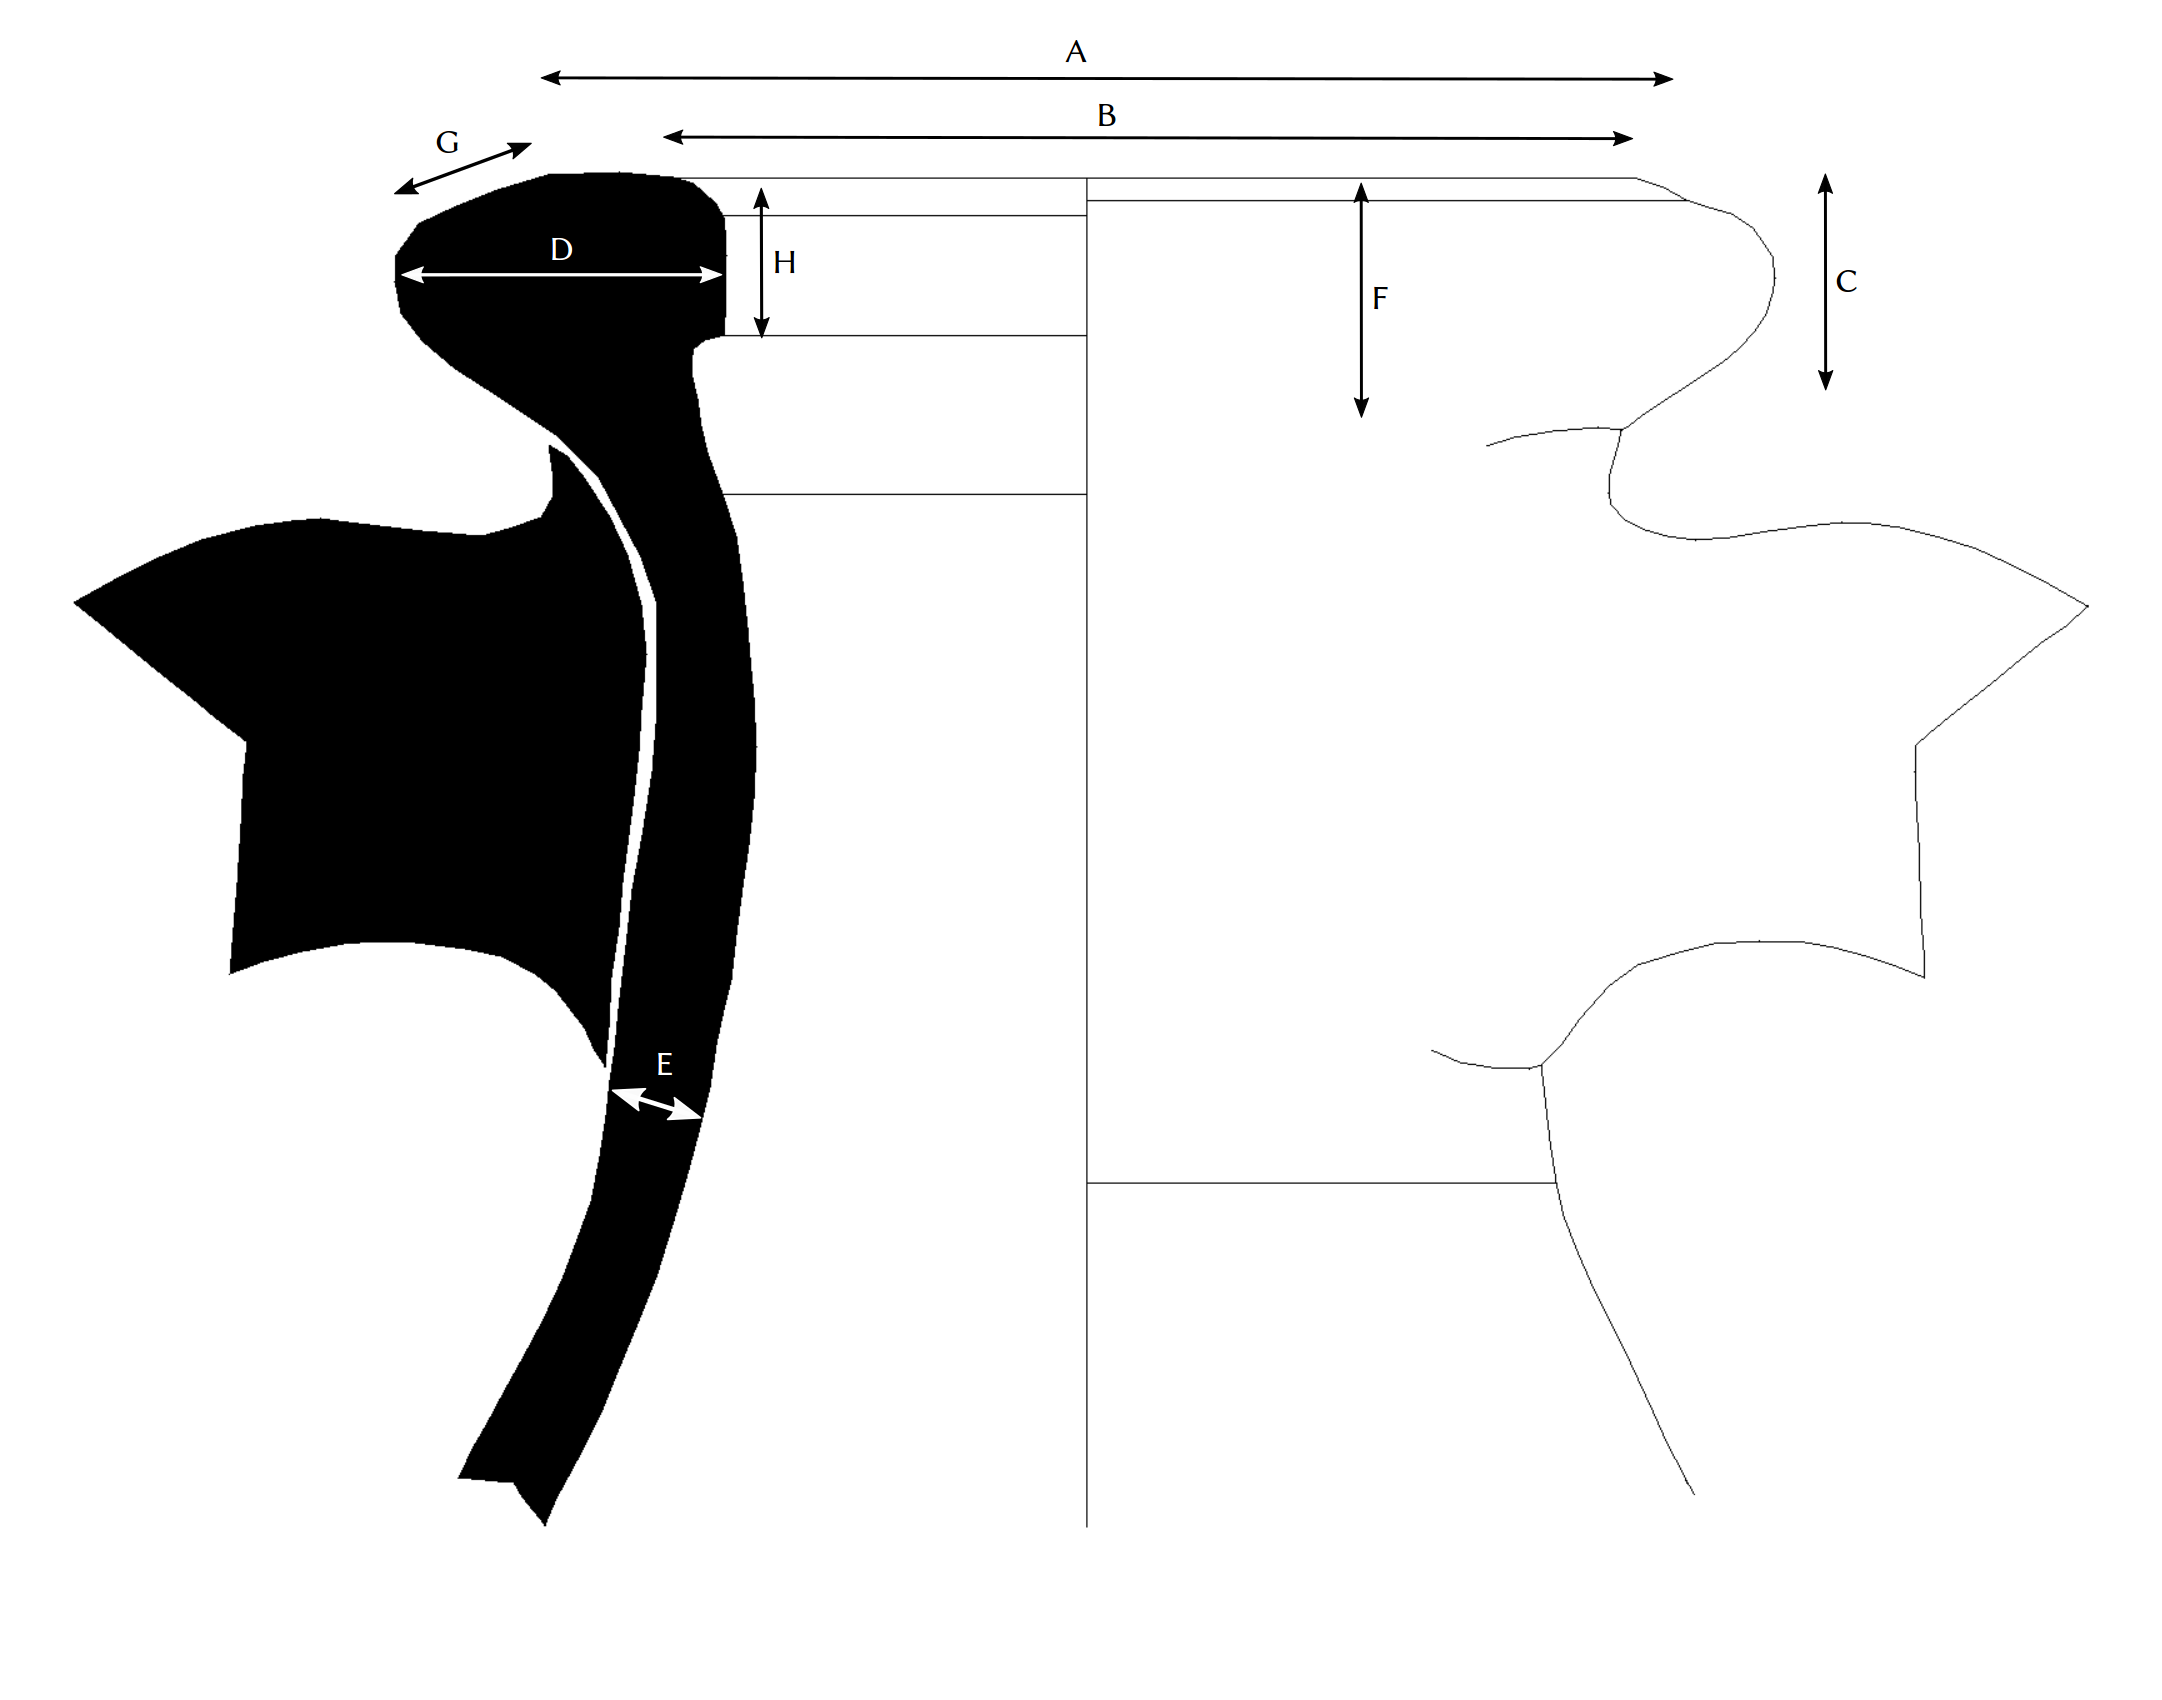
\includegraphics[width=\linewidth]{figs/mesures.png}
\caption{The 8 morphometric measurements taken for all amphorae. A: External diameter. B: Inside diameter. C: Rim height. D: Rim width. E: Shape width. F: Rim inside height. G: Rim width 2. H: Protruding rim}
\label{mesures}
\end{figure} 
 

\subsection{Principal Component Analysis}

Principal Component Analysis (PCA) was used to simplify the large number of variables in our dataset. The method allowed us to synthetise the data by focusing on a small number of Principal Components (PCs) while retaining a majority of the variation which was in essence what we wanted to explore \citep{jolliffe_principal_2002}. PCA is a common method in archaeology in scenarios studying intrasample veriation \citep{ shennan_quantifying_1997, li_crossbows_2014, schillinger_differences_2016}.

%In order to apply a degree of uniformity, we created a training dataset of 210 samples. In our study, PCA allowed to capture the most variation of the measurement and retained into first two principal components. 

%The new set of variables contain all the relevant information of the previous variables without losing relevance. The first principal components are expressed as the result of the most variance of the all information from the original variables. Moreover the information is expressed as the result of most variation retained in the first principal components \citep{jolliffe_principal_2002, shennan_quantifying_1997}. of the measurements and  into PCs and take the first PCA with more variability in the dataset. 

\subsection{Discriminant Linear Analysis} 

The next step was focused on evaluating if differences in the two main Principal Components are linked to the workshop where the amphorae were made. This idea was explored with the application of clustering algorithm and the evaluation of a Confusion Matrix. If the amphorae made in two workshops are easily confused then their average measures are similar; on the other hand, if the rate of misclassification between two workshops is very low then the amphorae made in these locations are distinctively different. 

The choice of clustering method was Linear Discriminant Analysis (LDA). Training was performed using a randomly sampled dataset with equal sample size for each workshop. The trained LDA model was then applied to the entire dataset as we were interested on how well workshop attribution could be predicted relying exclusively on morphometric measures. A Confusion Matrix (CM) was used to quantify under what extent the amphorae of different workshops can be identified. CM computes this quantity as the probability of misclassification between each pair of groups in the dataset (e.g. the workshops). This method has already been used in similar scenarios aiming at identifying differences in artefact production \citep{charlton_investigating_2012, thorpe_distribution_1984,i_martin_alisis_1998}



%The variability of the first 2 Principal Components was used to cluster our dataset using Linear Discriminant Analysis (LDA). LDA was conducted to find significant differences among workshops by the combination among variables obtained for the first principal components. LDA identifies which variables allow to distinguish or discriminate each group and how many variables are necessary to achieve the best combination as possible. In our case, this method allowed to demonstrate the correlation between spatial distance and distance among workshops. LDA was used to explore a better separate training set from the results of the most relevant principal components. LDA can classify the PCs result of the measurements into different groups.  We also generate a Confusion Matrix (CM) to able of quantifying the degree of confusion and compare the index of similarity among workshops.  CM calculated the probability of success and error of the results. It generates a matrix where higher value are the results of an incorrect classification. The distance generated with the results of DA will be compared with the spatial distance to see if it exists a correlation between morphometric distance and spatial distance. As example, this method has been commonly used to detect differences in artifact production \citep{charlton_investigating_2012, thorpe_distribution_1984}, and particularly for a similar study about the production pottery in \emph{Tarraconense} \citep{i_martin_alisis_1998}


\subsection{Spatial Distance}

The last step of this method was the comparison of the similarity distance provided by the Confusion Matrix against the spatial distance between workshops. A significant correlation etween these distance matrices would suggest processes of isolation-by-distance typical from vertical transmission \citep{crema_culture_2014}. Euclidean distance was used to measure distance amongst workshops as they were aligned following the river course. The evaluation of these two distance matrices (morphometric distance and spatial distance) was computed using a Mantel test. Mantel test evaluates the degree of pairwise correlation between two matrices and has been particularly useful in archaeology to explore the spatial dimension of cultural change \citep{mantel_detection_1967, diniz-filho_mantel_2013, crema_culture_2014}.  


\section{Results}

The Principal Components of the dataset are listed in Table~\ref{table:variable}

\begin{table}[htp]
\begin{tabular}{lcccccccc}
\hline
 Variables		&    PC1 & PC2	& PC3 & PC4 & PC5 & PC6 & PC7 & PC8     \\ \hline
 Exterior diameter& 		 &-0.195	&	  &  	&0.281&-0.217&0.369&0.829           \\
 Inside diameter& 		 &		&0.105&-0.414&0.838&	    &-0.257&-0.202           \\
 Rim height&              &      &-0.143&-0.425&-0.242&-0.744&-0.424&           \\
 Rim width&       		 &-0.524	&0.136&  	&	  &-0.342&0.582&-0.497        \\
 Shape width&     		 &-0.170	&-0.920&0.253&0.232&		&     &          \\
 Rim inside&     		 &0.156 &-0.299&-0.750&-0.240&0.345&0.377&          \\                                    
 Rim width 2& 	         &-0.789	&	  &-0.113&-0.219	&0.393&-0.369&0.139          \\	
Protruding rim& \textbf{0.989} &      &      &     &     &     &     &          \\
\hline
\end{tabular}
\caption{PCA results. The \emph{Protruding rim} captures a majority of the variation.}
\label{table:variable}
\end{table}

Values for the two main Principal Components can be seen in Figure \ref{pca}. Exploratory analysis suggests that the second PC exhibit different dynamics for the most distant workshop (Parlamento). Additionally, the first PC also tends to display more similar values for amphorae made in nearby workshops such as Bel\'en and Malpica. 

\begin{figure}[htp]
	\centering
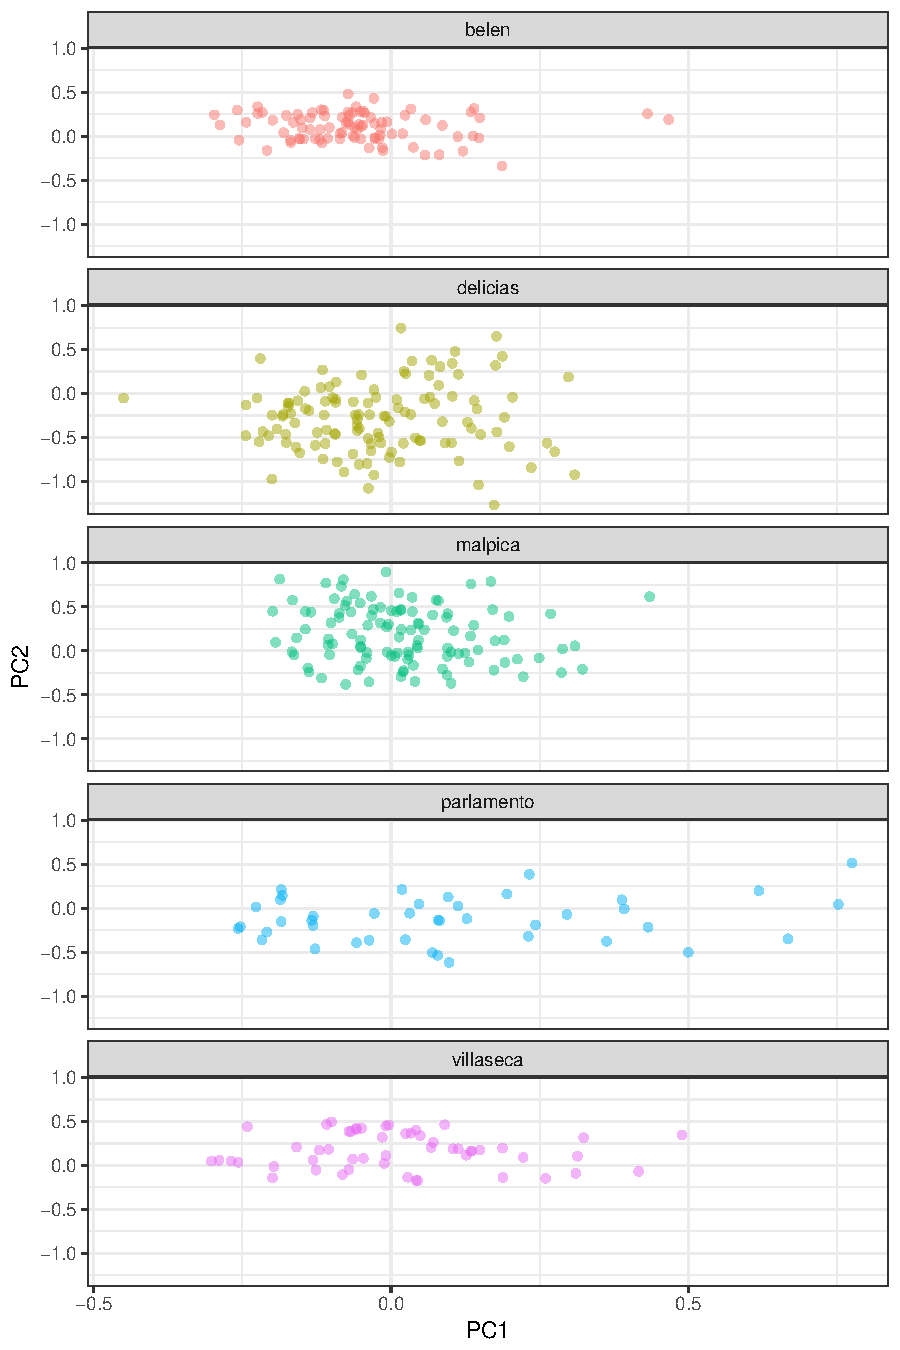
\includegraphics[width=\linewidth]{figs/pca}
\caption{Scatter plot for the First and Second PCs. Sample is split by workshop}
\label{pca}
\end{figure} 

\xavi{mirar AIXO!!!!}

LDA was applied to the two main PCs.  For the analysis, a total of 93 samples were correctly classified while 113 were incorrectly classified, as shown the Fig. \ref{prediction}. The results showed a similarity into three groups (Bel\'en, Malpica and Villaseca) while two groups depicted a different pattern (Las Delicias and Parlamento). This could be caused by the geographical proximity, being Parlamento and Las Delicias both workshops with the geographical distance more farther than rest of workshops. 



\begin{table}[htp]
\begin{tabular}{lccc}
\hline
      		&  PC1 & PC2	 \\ \hline
Standard Dev&0.3480758&0.1873301&\\
Proportion  &0.5747347&0.1664696&\\
Cumulative  &0.5747347&0.7412043& \\

\end{tabular}
\caption{Result values from the first two principal components}
\label{table:spatgeo}
\end{table}

Discriminant Analysis was used to analyse the results obtained from PCA.

\begin{figure}[htp]
	\centering
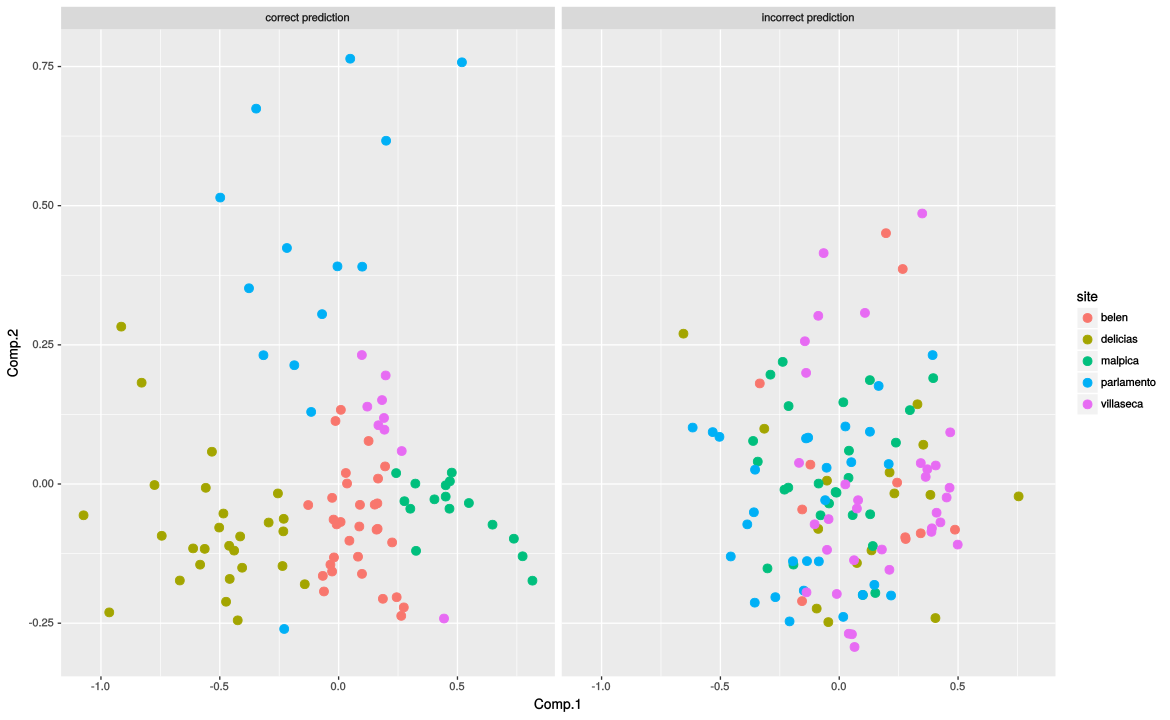
\includegraphics[width=\linewidth]{figs/prediction.png}
\caption{Plot with the correct and incorrect predictions result of Discriminant Analysis}
\label{prediction}
\end{figure} 

The results of Confusion Matrix proved that workshops with a minor spatial distance such as Malpica and Bel\'en had more troubles of being distinguished due to the similarity in the results obtained (see Table~\ref{table:confusion}). Classification test with the whole dataset gave an accuracy percentage of 50.61\%. Applying this to a training dataset reduced the accuracy to 46.19\%. Therefore, spatial distance could be inversely correlated with making techniques processes of amphorae in the case of \textit{Baetica} area. 

\begin{table}[htp]
\begin{tabular}{lccccc}
\hline
      & Bel\'en & Delicias & Malpica & Parlamento & Villaseca\\ \hline
Bel\'en &   31  &      6   &   12    &     11     &   13 \\
Delicias&  2  &     27   &    6    &     13     &    1  \\
Malpica &  6  &      4   &   16    &      2     &   13   \\
Parlamento & 3&      2   &   3     &      14    &    6    \\
Villaseca  & 0&      3   &    5    &      2     &    9     \\
\hline

\end{tabular}
\caption{Confusion Matrix with rows pointing out the workshops analysed. The sample analysed gave an accuracy percentage of 46.19 $\%$. Results of P.Value $<$0.01. }
\label{table:confusion}
\end{table}


 We calculated the correlation between spatial distance generated by the Euclidean distance and the distance among amphora measurements, calculated using the Confusion Matrix. The workshops were chosen with different geographical distance in order to prove the correlation between spatial distance and variability of the amphora production techniques. Mantel test indicated results more reasonable (rm= 0.3841; p= 0.025 with 199 permutations). The analysis shows that morphometric distance of the amphorae are strongly correlated with the spatial distance of workshops. Accordingly closer workshops tend to be more similar than the rest: when geographic distance is low, as the example of Bel\'en and Malpica, the morphometric distance seems more similar whereas when distance is higher, as Parlamento, the morphometric distance displays differences with the rest of workshops. Thus, the results suggest that the variability on the making-techniques processes might depend on the spatial distance.   


%\begin{table}[htp]
%\begin{tabular}{lccccc}
%\hline
%        & Bel\'en   &   Delicias & Malpica & Parlamento & Villaseca\\ \hline
%Bel\'en   &         &   0.8409091&0.7272727&0.7857143   &0.7169811  \\
%Delicias&0.8409091&            &0.7522523&0.7023810   &0.8018868   \\
%Malpica &0.7272727&0.7522523   &         &0.7142857   &0.6509434    \\
%Parlamento&0.7857143&0.7023810&0.7142857&            &0.7380952     \\
%Villaseca&0.7169811&0.8018868&0.6509434&0.7380952    &                \\
%\hline

%\end{tabular}
%\caption{Results of matrix distance among workshops}
%\label{table:spatialdistance}
%\end{table}

%\begin{figure}[htp]

 %\centerin
%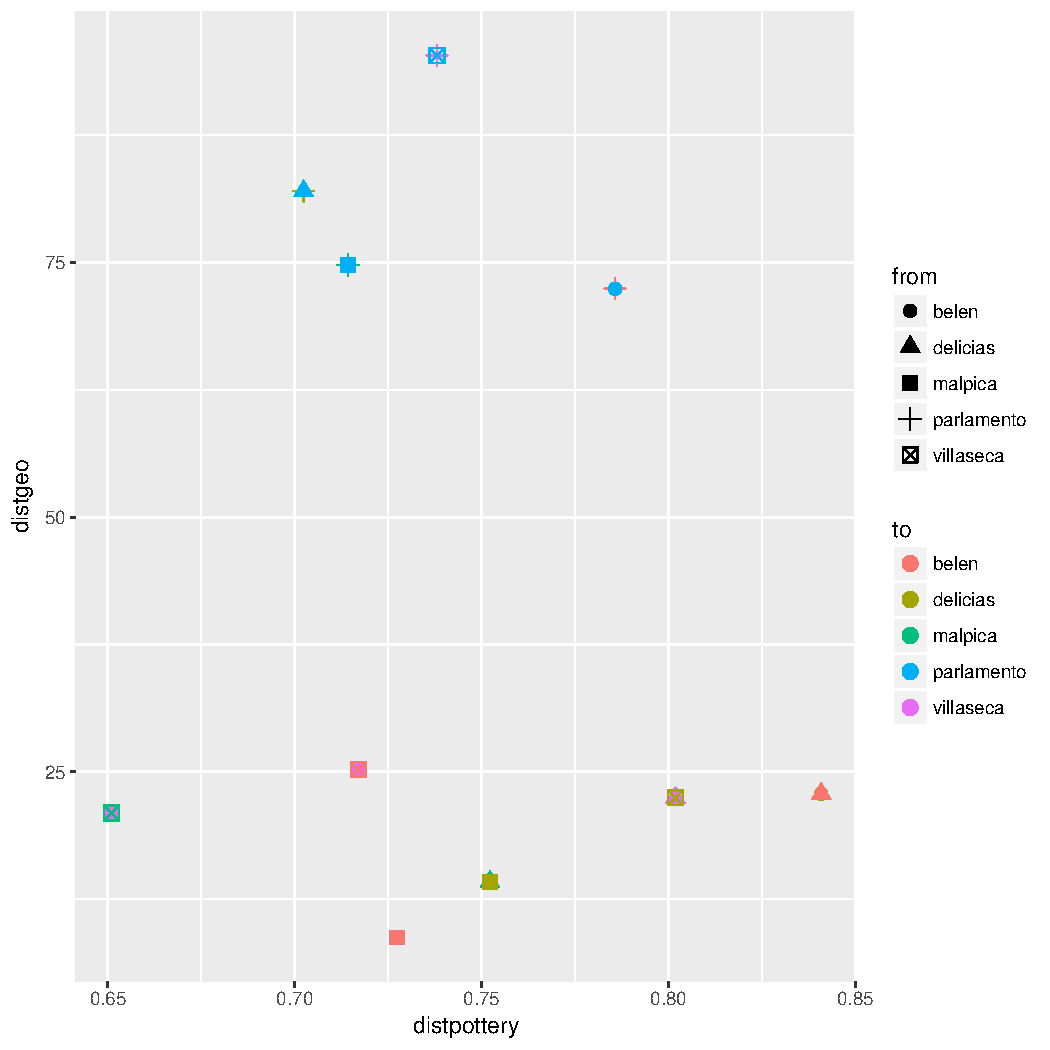
\includegraphics[scale=0.60]{spatgeo.pdf}
%\caption{Plot with the results of the comparison between morphometric distance (distpottery) and spatial distance (distgeo) in km}
%\label{spatgeo}
%\end{figure} 


%\begin{table}[htp]
%\begin{tabular}{llcc}
%\hline
% From		& To 		& Morphometric distance	& Geographic distance\\ %\hline
% Parlamento	& Belen		& 						&  72.45				 \\
% Parlamento	& Delicias	& 						&  82.01				 \\
 %Parlamento	& Malpica   &                       	&  74.77                      \\
 %Parlamento	& Villaseca	&						&  95.33					\\
 %Belen		& Parlamento &						&  72.45						\\
 %Belen		& Delicias   &						&  22.82      				 \\                                    
 %Belen		& Malpica	&						&  8.73							%\\	
 %Belen		& Villaseca  &                       &  25.23                         \\
 %Delicias	& Parlamento  &                      &  82.01                            \\
 %Delicias	& Belen       &						&  22.82						\\
 %Delicias	& Malpica     &						&  14.19						\\
 %Delicias	& Villaseca   &						&  22.45						\\
 %Malpica		& Parlamento  &						&  74.77						\\
 %Malpica		& Belen       &						&  8.73						\\
 %Malpica		& Delicias    &						&  14.19						\\
 %Malpica    & Villaseca	  &						&  20.97                     \\
 %Villaseca	& Belen       &						&  25.23					     \\Villaseca	& Malpica     &		                 &  20.97			
 %\\
 %Villaseca	& Delicias	  &						&  22.45								\\
 %Villaseca	& Parlamento	  &						&  95.33								\\
                                                   
%\hline

%\end{tabular}
%\caption{Results with the comparison between morphometric distance and geographic distance (km) }
%\label{table:spatgeo}
%\end{table}


\section{Discussion and Conclusion}

Differences on the making techniques processes among workshops show a variability correlated with spatial distance. The analysed morphometric traits suggest that the similarity between amphorae decreases with the spatial distance between the workshops where they were produced. As a result, amphorae made in nearby workshops with a minor spatial distance share more traits than amphorae made in pottery workshops farthest. In other words, the variability on the making techniques processes was more difficult to differentiate in nearest workshops. In our case, Malpica and Bel\'en workshops where the geographical proximity is the closest shared more traits in comparison with other workshops (Parlamento and Las Delicias). Thus the probability of interaction between workshops is increasing when the proximity is closest while this likelihood decreases when the possibility of interaction is low. 

We have observed than rivers courses could have affected in the transmission factors. In the case of the commerce, rivers and its tributaries played an important role for the transport of goods. The huge demand within Roman Empire and the good conditions for the loading and unloading of products \citep{bevan_mediterranean_2014} might have influenced the mode of transmission due to the continuous contact between workshops. 

The results also suggest that vertical transmission could be the main cultural mechanism to explain the variability between workshops. The different morphological traits among workshops seem proper of a low contact between potters from other workshops. The evidence confirms therefore that these pottery techniques were transmitted with high fidelity and few changes during three centuries. It would mean that the disciples could have remained the learning techniques in the workshops where they were trained. By contrast, horizontal transmission doesn't seem to be the most probable process. The continuous contact between potters from different places generated a greater homogeneity in the technical practises. As results, workshops were sharing the same production techniques that it would generate a social network where potters within the same generation worked in different workshops at the same time. Our result suggest a progressive contact with closer workshops instead. Moreover, the fact that isolation by distance is detected suggests a limited displacement between distant workshops. Thus, vertical transmission would be explained with this observed process. However, the diversity of social learning processes are clearly complex. In other words, the transmission of technical skills between master and disciple did not discard that horizontal transmission played an important role in this process as well. It can be a process where this vertical transmission dominated at first in the same workshops but consequently this transmission would be affected by workers who exchanged ideas or workers moving to other workshops. 

The combination of empirical analysis with statistical method have provided a strong baseline for a better understanding of the amphora production in the Roman Empire. These methods offer also an alternative complement to other methods as archaeometry for the characterization of production sites and places of consumption. We have identified measurable differences in the techniques by observing and we have tested those particularities using multivariate methods and Mantel test. Our analysis provides a useful guideline for the exploration of the social learning processes related with amphora production in the Roman Empire. Hence, the results have lightened to understand the link between social learning and archaeological evidence in a diversity of scenarios. 

\section{Acknowledgments}

The research was funded by European Research Council Advanced Grant EPNet (340828). We are grateful to Enrique Garc\'ia Vargas and Simon Carrignon for helpful suggestions and constructive comments on previous versions of the paper. The Museum of \'Ecija (Antonio Fern\'andez Ugalde), Museum of Palma del R\'io (Reyes Lopera and Emilio Navarro), Museum of C\'ordoba and Museum of Seville for kindly allowing us access to their information.  
Data were collected, performed and analysed in R version 3.2.4. statistical language and implemented with the package MASS and vegan. Map was done by QGIS 2.8 Wien with Pleiades template. 



\section*{References}

%\bibliographystyle{apalike}
\bibliography{mybibfile}

\end{document}

\cite
